%\chapter{Main Results}
\chapter{実験}

\section{実験環境、前提}

実験環境として、2次元の有限な擬似連続空間とし、被動作対象であるトラジェクタと、参照点となりうる少量の物体が存在する空間内での物体移動動作の学習と再現、識別を行うシミュレータ環境を準備した。被教示者にとって、空間の範囲、トラジェクタや物体の数、位置、観点の種類は既知で教示者と認識を共有しており、各動作における観点については未知であるとし、その観点を教示動作から獲得し、動作の再現と識別を行うことを目標とする。
%%%%%%%%%%%%%%%%%%%%%%%%%%%%%%%%%%%%%%%%%%%%%%%%%%%%%%%%%%%%%%%%%%%%%%%%%%%%%%%%%%%%%%%%%%%%%%%%%%%%%%%
	\begin{figure}[b]
%中央ぞろえ
		\begin{center}
			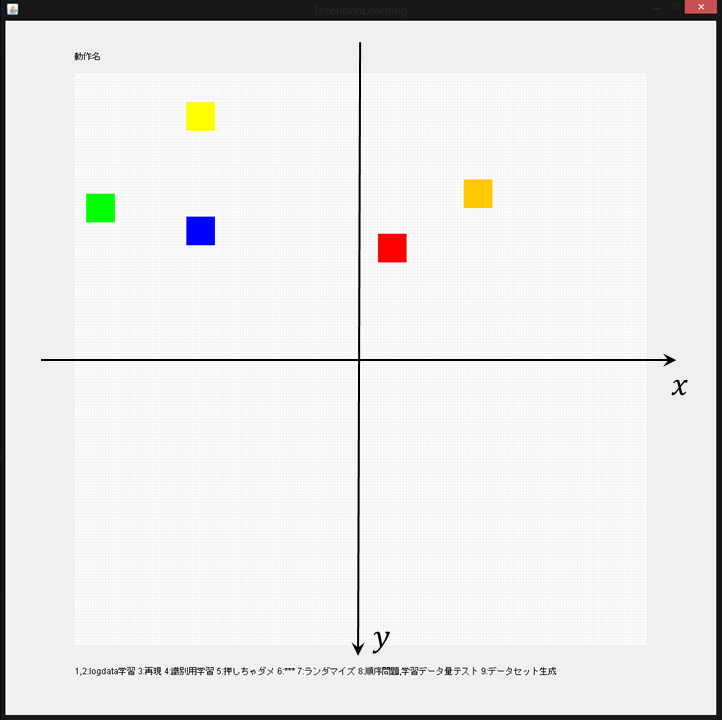
\includegraphics[width=8cm]{figure3.png} \\ %TeXの基本として, \\ で緊急改行ができる。(今回の場合や行列などを除き、あまり使わない)
			\caption{シミュレータ}
		\end{center}
	\end{figure}
%%%%%%%%%%%%%%%%%%%%%%%%%%%%%%%%%%%%%%%%%%%%%%%%%%%%%%%%%%%%%%%%%%%%%%%%%%%%%%%%%%%%%%%%%%%%%%%%%%%%%%%

\begin{table}[h]
	\caption{動作名とトラジェクタ目標位置の対応表}
	\label{table:taskname_15}
  	\begin{tabular}{|l|l|} \hline
    	動作名 & トラジェクタ目標位置\\ \hline
   	$T_{1}$ : 赤を中央に移動する & 
	$
    	\left( x_{center} , y_{center} \right)+G_{error}
    	$
    	\\
    	$T_{2}$ : 赤を青の右に移動する & 
	$
    	\left( x_{blue}+15 , y_{blue} \right)+G_{error}
    	$
    	\\
    	$T_{3}$ : 赤を橙の右に移動する & 
	$
    	\left( x_{orange}+15 , y_{orange} \right)+G_{error}
    	$
    	\\
    	$T_{4}$ : 赤を緑の右に移動する & 
	$
    	\left( x_{green}+15 , y_{green} \right)+G_{error}
    	$
    	\\
    	$T_{5}$ : 赤を黄の右に移動する & 
	$
    	\left( x_{yellow}+15 , y_{yellow} \right)+G_{error}
    	$
    	\\
    	$T_{6}$ : 赤を青に近づける & 
	$
    	\left( \frac{x_{red}+x_{blue}}{2} , \frac{y_{red}+y_{blue}}{2} \right)+G_{error}
    	$
    	\\
    	$T_{7}$ : 赤を橙に近づける & 
	$
    	\left( \frac{x_{red}+x_{orange}}{2} , \frac{y_{red}+y_{orange}}{2} \right)+G_{error}
    	$
    	\\
    	$T_{8}$ : 赤を緑に近づける & 
	$
    	\left( \frac{x_{red}+x_{green}}{2} , \frac{y_{red}+y_{green}}{2} \right)+G_{error}
    	$
    	\\
    	$T_{9}$ : 赤を黄に近づける & 
	$
    	\left( \frac{x_{red}+x_{yellow}}{2} , \frac{y_{red}+y_{yellow}}{2} \right)+G_{error}
    	$
    	\\
    	$T_{10}$ : 赤を青から遠ざける & 
	$
    	\left( 2x_{red}-x_{blue} , 2y_{red}-y_{blue} \right)+G_{error}
    	$
    	\\
    	$T_{11}$ : 赤を橙から遠ざける & 
	$
    	\left( 2x_{red}-x_{orange} , 2y_{red}-y_{orange} \right)+G_{error}
    	$
    	\\
    	$T_{12}$ : 赤を緑から遠ざける & 
	$
    	\left( 2x_{red}-x_{green} , 2y_{red}-y_{green} \right)+G_{error}
    	$
    	\\
    	$T_{13}$ : 赤を黄から遠ざける & 
	$
    	\left( 2x_{red}-x_{yellow} , 2y_{red}-y_{yellow} \right)+G_{error}
    	$
    	\\
    	$T_{14}$ : 等間隔に赤、黄、青と並べる & 
	$
    	\left( 2x_{yellow}-x_{blue} , 2y_{yellow}-y_{blue} \right)+G_{error}
    	$
    	\\
    	$T_{15}$ : 時計回りに赤、緑、青と並べる & 
	$
	\begin{pmatrix}
        	\cos \frac{\pi}{3} & -\sin \frac{\pi}{3} \\
        	\sin \frac{\pi}{3} & \cos \frac{\pi}{3}
	\end{pmatrix}
	\begin{pmatrix}
        	x_{blue}-x_{green} \\
        	y_{blue}-y_{green}
	\end{pmatrix}
      	+
	\begin{pmatrix}
        	x_{green} \\
        	y_{green}
	\end{pmatrix}      	
	+G_{error}
    	$
    	\\ \hline
  	\end{tabular}
\end{table}
また本実験において使用した動作の、動作名とその動作におけるトラジェクタの目標位置をまとめた表をTable \ref{table:taskname_15}に示す。
ただし、Table \ref{table:taskname_15}における$G_{error}$とは平均0のガウス分布から生起される誤差であり、分散の大きさは各実験ごとに設定する。$G_{error}$は教示誤差を表し、分散が小さいほど正確に与えられた教示動作となる。


\section{動作再現}

観点がコンピュータにとって未知である教示動作を与え、観点を推定し動作を再現する実験を行った。
実験にはTable \ref{table:taskname_15}の15動作のうち、赤を中央に移動する、赤を青の右に動かす、赤を橙に近づける、赤を緑から遠ざける、等間隔に赤、黄、青と並べる、時計回りに赤、緑、青と並べるの6動作を使用した。
教示時の誤差(教示誤差)をガウス誤差の分散0.5間隔で0から20まで増やしながらそれぞれ500データ生成し、10データ1セットの一つ抜き法で再現時の誤差(再現誤差)の計算を各教示誤差で計50回ずつ行った。計算結果を付録\ref{appendix1}に示す。
観点推定の成否の判定は計算結果のうち各教示誤差における標準偏差の2.896倍以上の誤差が生じた再現結果を推定失敗と定めた。Fig.\ref{figure:success_rate}に、そのようにして各再現結果を成功と失敗に分けた観点推定の正答率のグラフを示す。また付録\ref{appendix2}に、各教示誤差と再現誤差の関係と、判定基準を上記のように定められることの詳細を示す。
%%%%%%%%%%%%%%%%%%%%%%%%%%%%%%%%%%%%%%%%%%%%%%%%%%%%%%%%%%%%%%%%%%%%%%%%%%%%%%%%%%%%%%%%%%%%%%%%%%%%%%%
	\begin{figure}[h]
%中央ぞろえ
		\begin{center}
			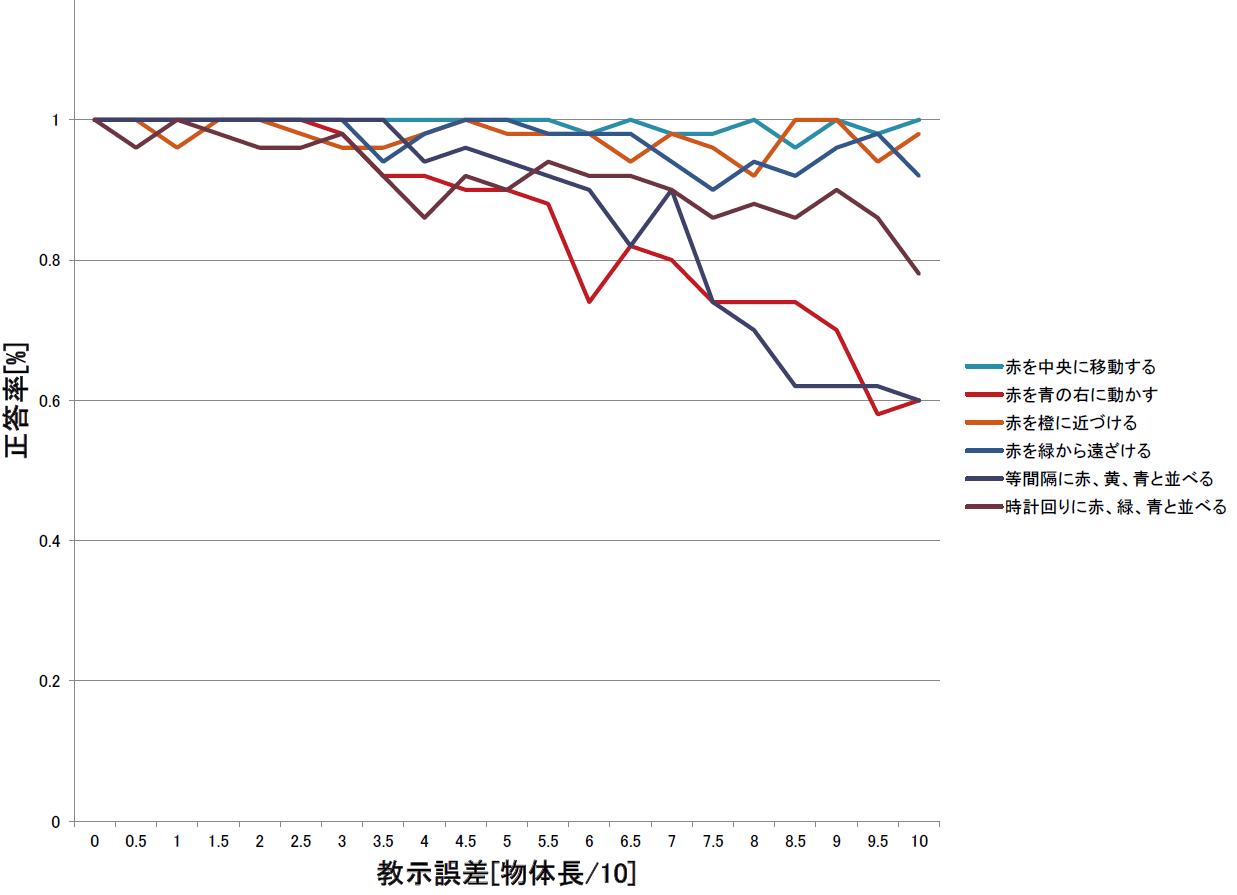
\includegraphics[width=14cm]{chart2.png} \\ %TeXの基本として, \\ で緊急改行ができる。(今回の場合や行列などを除き、あまり使わない)
			\caption{教示誤差と正答率の関係のグラフ}
			\label{figure:success_rate}
		\end{center}
	\end{figure}
%%%%%%%%%%%%%%%%%%%%%%%%%%%%%%%%%%%%%%%%%%%%%%%%%%%%%%%%%%%%%%%%%%%%%%%%%%%%%%%%%%%%%%%%%%%%%%%%%%%%%%%

Fig.\ref{figure:success_rate}から、教示時の誤差が十分に小さい場合に、観点の推定が適切に行えていることがわかる。また、等間隔に赤、黄、青と並べる動作、時計回りに赤、緑、青と並べる動作においても適切に再現できていることから、複数の参照点を含む動作を適切に学習できていることがわかる。実験に使用した動作のうち、中央に移動する動作、橙に近づける動作、緑に近づける動作の正答率が意図した状態と異なり、教示誤差の増加に無関係に再現できているが、これは学習時の遷移ベクトルの正規化長に依るものだと考えられる。また中央に移動する動作は中央に近づける動作とも認識できる等、適切な観点モデルが複数存在する動作に関して誤答率が下がったとも考えられる。




\section{動作識別}

動作名が未知である例示動作を与え、それが既学習動作のうちいずれであるかを推定する実験を行った。
既学習動作はTable \ref{table:taskname_15}の15動作とし、
各動作において教示動作として分散3のガウス誤差を持つ30データを生成し学習を行った。例示動作は動作再現実験と同様のの6動作を使用し、各動作分散10のガウス誤差を持つ100データを生成してテストを行った。Table \ref{table:result}に各例示動作の識別正答率を示す。
\begin{table}[h]
	\caption{動作識別の正答率}
	\label{table:result}
	\centering
  	\begin{tabular}{|l|l|} \hline
    	動作名 & 正答率\\ \hline
   	赤を中央に移動する 		& 0.96
    	\\
    	赤を青の右に移動する 		& 0.98
    	\\
    	赤を橙に近づける 			& 0.97
    	\\
    	赤を緑から遠ざける 			& 0.97
    	\\
    	等間隔に赤、黄、青と並べる 	& 1.00
    	\\
    	時計回りに赤、緑、青と並べる 	& 0.96
    	\\ \hline
  	\end{tabular}
\end{table}
Table \ref{table:result}より、学習済みの動作に関して例示動作の識別が適切に行えていることがわかる。また、誤識別が生じた初期環境と例示動作の例をFig.\ref{figure:failure}に示す。例えばFig.\ref{figure:failure}左は赤を橙に近づける例示動作だが、赤を緑から遠ざける動作だと誤って識別されている。誤識別が生じた例示動作に関しては、多くがこのように人間にとっても適切な動作が判別しづらいものであった。


%%%%%%%%%%%%%%%%%%%%%%%%%%%%%%%%%%%%%%%%%%%%%%%%%%%%%%%%%%%%%%%%%%%%%%%%%%%%%%%%%%%%%%%%%%%%%%%%%%%%%%%
%Fig.が入れらんねぇ

	\begin{figure}[h]
%中央ぞろえ
		\begin{center}
			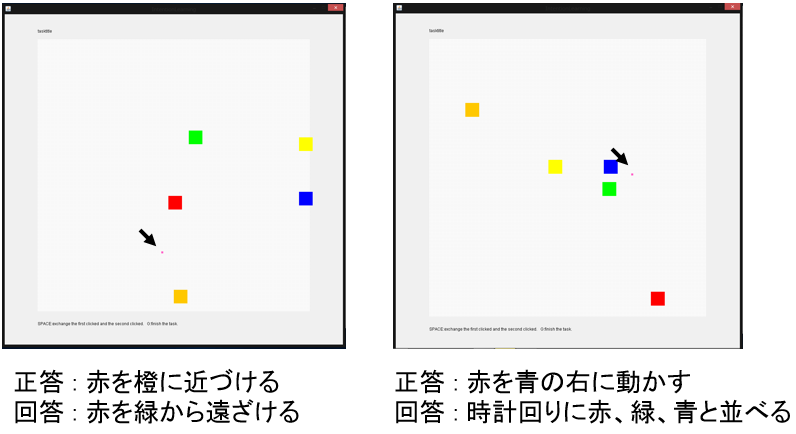
\includegraphics[width=10cm]{figure4.png} \\ %TeXの基本として, \\ で緊急改行ができる。(今回の場合や行列などを除き、あまり使わない)
			\caption{誤識別例}
			\label{figure:failure}
		\end{center}
	\end{figure}

%%%%%%%%%%%%%%%%%%%%%%%%%%%%%%%%%%%%%%%%%%%%%%%%%%%%%%%%%%%%%%%%%%%%%%%%%%%%%%%%%%%%%%%%%%%%%%%%%%%%%%%
